% Options for packages loaded elsewhere
\PassOptionsToPackage{unicode}{hyperref}
\PassOptionsToPackage{hyphens}{url}
%
\documentclass[]{article}
\usepackage{amsmath,amssymb}
\usepackage{lmodern}
\usepackage{iftex}
\ifPDFTeX
  \usepackage[T1]{fontenc}
  \usepackage[utf8]{inputenc}
  \usepackage{textcomp} % provide euro and other symbols
\else % if luatex or xetex
  \usepackage{unicode-math}
  \defaultfontfeatures{Scale=MatchLowercase}
  \defaultfontfeatures[\rmfamily]{Ligatures=TeX,Scale=1}
\fi
% Use upquote if available, for straight quotes in verbatim environments
\IfFileExists{upquote.sty}{\usepackage{upquote}}{}
\IfFileExists{microtype.sty}{% use microtype if available
  \usepackage[]{microtype}
  \UseMicrotypeSet[protrusion]{basicmath} % disable protrusion for tt fonts
}{}
\makeatletter
\@ifundefined{KOMAClassName}{% if non-KOMA class
  \IfFileExists{parskip.sty}{%
    \usepackage{parskip}
  }{% else
    \setlength{\parindent}{0pt}
    \setlength{\parskip}{6pt plus 2pt minus 1pt}}
}{% if KOMA class
  \KOMAoptions{parskip=half}}
\makeatother
\usepackage{xcolor}
\IfFileExists{xurl.sty}{\usepackage{xurl}}{} % add URL line breaks if available
\IfFileExists{bookmark.sty}{\usepackage{bookmark}}{\usepackage{hyperref}}
\hypersetup{
  pdftitle={arc42 Template},
  hidelinks,
  pdfcreator={LaTeX via pandoc}}
\urlstyle{same} % disable monospaced font for URLs
\usepackage{longtable,booktabs,array}
\usepackage{calc} % for calculating minipage widths
% Correct order of tables after \paragraph or \subparagraph
\usepackage{etoolbox}
\makeatletter
\patchcmd\longtable{\par}{\if@noskipsec\mbox{}\fi\par}{}{}
\makeatother
% Allow footnotes in longtable head/foot
\IfFileExists{footnotehyper.sty}{\usepackage{footnotehyper}}{\usepackage{footnote}}
\makesavenoteenv{longtable}
\usepackage{graphicx}
\makeatletter
\def\maxwidth{\ifdim\Gin@nat@width>\linewidth\linewidth\else\Gin@nat@width\fi}
\def\maxheight{\ifdim\Gin@nat@height>\textheight\textheight\else\Gin@nat@height\fi}
\makeatother
% Scale images if necessary, so that they will not overflow the page
% margins by default, and it is still possible to overwrite the defaults
% using explicit options in \includegraphics[width, height, ...]{}
\setkeys{Gin}{width=\maxwidth,height=\maxheight,keepaspectratio}
% Set default figure placement to htbp
\makeatletter
\def\fps@figure{htbp}
\makeatother
\setlength{\emergencystretch}{3em} % prevent overfull lines
\providecommand{\tightlist}{%
  \setlength{\itemsep}{0pt}\setlength{\parskip}{0pt}}
\setcounter{secnumdepth}{-\maxdimen} % remove section numbering
\ifLuaTeX
  \usepackage{selnolig}  % disable illegal ligatures
\fi

\title{
Implementation of Cloud Transformation Scenario \\
Frankfurt University of Applied Sciences \\
Module: Cloud Computing - Milestone 3
}

\date{January, 28th 2025}

\begin{document}

\begin{flushleft}
Frankfurt University of Applied Sciences\\
Fachbereich 2: Informatik und Ingenieurwissenschaften\\
Allgemeine Informatik (M.Sc.) / High Integrity Systems (M.Sc.)\\
\end{flushleft}

\vspace{3.5cm}

\begin{center}
    \Large
    \textbf{Cloud Computing Project} \\
    \Large
    Milestone 3 - Implementation of Cloud Transformation Scenario
\end{center}

\vspace{2cm}

\begin{center}
    Edward Späth - 1386244 \\
    Dennis Mark - 1384589 \\ 
    Vinay Duhan - 1475786 \\
    Jatender Singh Jossan - 1346747 \\
    Dominique Conceicao Rosario — 1399464
\end{center}

\vspace{6.7cm}

\begin{flushright}
    Lecturer: Henry-Norbert Cocos\\
    Course: Cloud Computing\\
    Winter Semester 24/25\\
\end{flushright}

\tableofcontents

\newpage

\listoffigures

\newpage

\hypertarget{section-introduction-and-goals}{%
\section{Introduction and Goals}\label{section-introduction-and-goals}}

Describes the relevant requirements and the driving forces that software
architects and development team must consider. These include

\begin{itemize}
\item
  underlying business goals,
\item
  essential features,
\item
  essential functional requirements,
\item
  quality goals for the architecture and
\item
  relevant stakeholders and their expectations
\end{itemize}

\hypertarget{_requirements_overview}{%
\subsection{Requirements Overview}\label{_requirements_overview}}

\textbf{Contents}

Short description of the functional requirements, driving forces,
extract (or abstract) of requirements. Link to (hopefully existing)
requirements documents (with version number and information where to
find it).

\textbf{Motivation}

From the point of view of the end users a system is created or modified
to improve support of a business activity and/or improve the quality.

\textbf{Form}

Short textual description, probably in tabular use-case format. If
requirements documents exist this overview should refer to these
documents.

Keep these excerpts as short as possible. Balance readability of this
document with potential redundancy w.r.t to requirements documents.

See \href{https://docs.arc42.org/section-1/}{Introduction and Goals} in
the arc42 documentation.

\hypertarget{_quality_goals}{%
\subsection{Quality Goals}\label{_quality_goals}}

\textbf{Contents}

The top three (max five) quality goals for the architecture whose
fulfillment is of highest importance to the major stakeholders. We
really mean quality goals for the architecture. Don't confuse them with
project goals. They are not necessarily identical.

Consider this overview of potential topics (based upon the ISO 25010
standard):

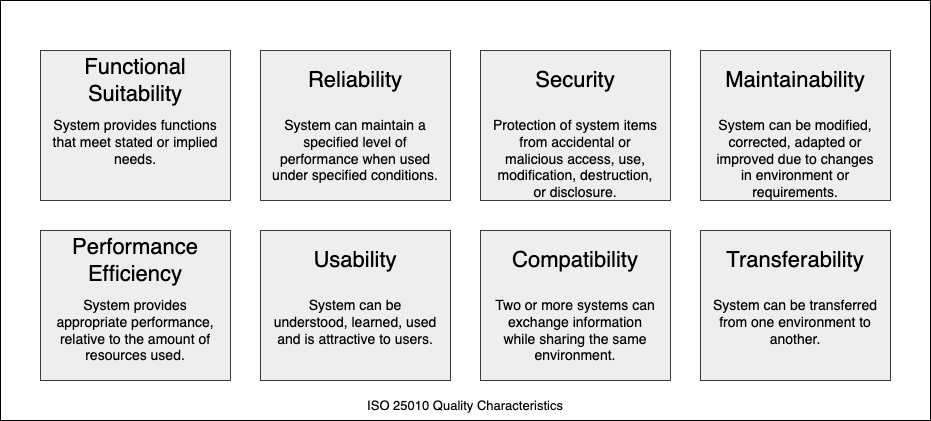
\includegraphics{images/01_2_iso-25010-topics-EN.drawio.png}

\textbf{Motivation}

You should know the quality goals of your most important stakeholders,
since they will influence fundamental architectural decisions. Make sure
to be very concrete about these qualities, avoid buzzwords. If you as an
architect do not know how the quality of your work will be
judged\ldots{}

\textbf{Form}

A table with quality goals and concrete scenarios, ordered by priorities

\hypertarget{_stakeholders}{%
\subsection{Stakeholders}\label{_stakeholders}}

\textbf{Contents}

Explicit overview of stakeholders of the system, i.e. all person, roles
or organizations that

\begin{itemize}
\item
  should know the architecture
\item
  have to be convinced of the architecture
\item
  have to work with the architecture or with code
\item
  need the documentation of the architecture for their work
\item
  have to come up with decisions about the system or its development
\end{itemize}

\textbf{Motivation}

You should know all parties involved in development of the system or
affected by the system. Otherwise, you may get nasty surprises later in
the development process. These stakeholders determine the extent and the
level of detail of your work and its results.

\textbf{Form}

Table with role names, person names, and their expectations with respect
to the architecture and its documentation.

\begin{longtable}[]{@{}
  >{\raggedright\arraybackslash}p{(\columnwidth - 4\tabcolsep) * \real{0.2000}}
  >{\raggedright\arraybackslash}p{(\columnwidth - 4\tabcolsep) * \real{0.4000}}
  >{\raggedright\arraybackslash}p{(\columnwidth - 4\tabcolsep) * \real{0.4000}}@{}}
\toprule
\begin{minipage}[b]{\linewidth}\raggedright
Role/Name
\end{minipage} & \begin{minipage}[b]{\linewidth}\raggedright
Contact
\end{minipage} & \begin{minipage}[b]{\linewidth}\raggedright
Expectations
\end{minipage} \\
\midrule
\endhead
\emph{\textless Role-1\textgreater{}} &
\emph{\textless Contact-1\textgreater{}} &
\emph{\textless Expectation-1\textgreater{}} \\
\emph{\textless Role-2\textgreater{}} &
\emph{\textless Contact-2\textgreater{}} &
\emph{\textless Expectation-2\textgreater{}} \\
\bottomrule
\end{longtable}
\newpage
\section{Constraints}

\subsection{Technical Constraints}
The Webshop system is built with the following fixed technologies:

\begin{table}[h]
\centering
\begin{tabular}{|l|l|}
\hline
\textbf{Category} & \textbf{Chosen Technology} \\ \hline
\textbf{Frontend} & Next.js (React Framework) with Tailwind CSS \\ \hline
\textbf{Backend} & Python Flask (REST API implementation) \\ \hline
\textbf{Database} & Microsoft Azure SQL Database \\ \hline
\textbf{Storage} & Azure Blob Storage for product images \\ \hline
\textbf{Hosting} & Azure App Services and Azure Container Apps \\ \hline
\textbf{Authentication} & No authentication required (demo version) \\ \hline
\textbf{Version Control} & GitHub repository with structured commit history \\ \hline
\textbf{Scalability} & Azure auto-scaling and load balancing \\ \hline
\end{tabular}
\caption{Technical Constraints for Webshop Development}
\label{tab:constraints}
\end{table}

\subsection{Organizational Constraints}
\begin{itemize}
    \item \textbf{Cloud Provider:} The project is hosted on \textbf{Microsoft Azure}.
\end{itemize}

\newpage
\hypertarget{section-system-scope-and-context}{%
\section{System Scope and Context}\label{section-system-scope-and-context}}

\textbf{Contents}

This section defines the scope and context of the Webshop system, a platform designed to display products to users, process payments, and confirm orders. The system retrieves product data from an Azure-hosted database, integrates with Stripe for payment processing, and uses an Azure email service to send order confirmations. It outlines the external entities users, the Azure database, Stripe, and the Azure email service and specifies the business and technical interfaces connecting them to the Webshop.

\textbf{Motivation}

Understanding the Webshop's and its external entities interfaces is crucial for stakeholders to make informed architectural decisions. Clear boundaries ensure alignment on what the system handles (e.g., product display and payment) versus what it relies on externally (e.g., payment processing via Stripe), guiding both development and deployment decisions.

\textbf{Form}

The business context will be presented with a context diagram showing the Webshop as a black box linked to its external partners, a table listing communication partners, inputs, and outputs. The technical context will use a UML deployment diagram to illustrate the system’s technical connections, supplemented by a mapping table tying domain inputs/outputs to specific channels.

\hypertarget{_business_context}{%
\subsection{Business Context}\label{_business_context}}

\textbf{Contents}

The Webshop system interacts with several external entities: (1) Users, who browse products, submit orders, provide payment information, and receive order confirmations; (2) Azure-hosted Database, which provides product data; (3) Stripe, which processes payment transactions; and (4) Azure Email Service, which delivers order confirmation emails. This subsection specifies the domain-specific inputs and outputs exchanged between the Webshop and these partners.

\textbf{Motivation}

Defining these interactions ensures stakeholders understand the Webshop’s core business functions displaying products, processing orders, and confirming purchases and its dependencies on external systems for data, payments, and notifications.

\textbf{Form}

The context diagram below depicts the Webshop system and its external interactions. The table details the inputs and outputs for each communication partner.

\begin{figure}[h]
  \centering
  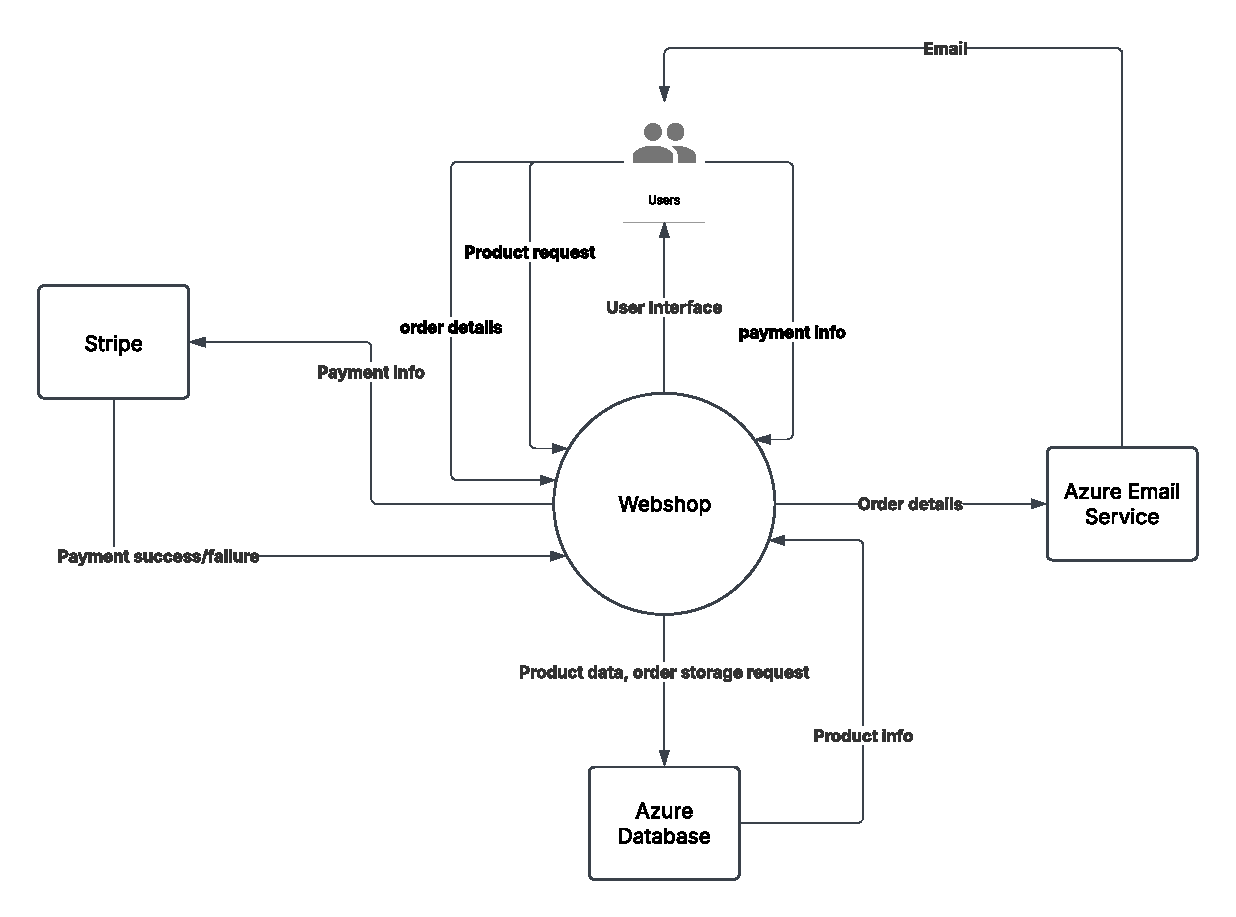
\includegraphics[width=0.8\textwidth]{images/webshop_context_diagram.pdf} 
  \caption{Context Diagram of the Webshop System and Its External Entities}
  \label{fig:webshop-context}
\end{figure}

\begin{table}[h]
  \centering
  \resizebox{\textwidth}{!}{%
    \begin{tabular}{|l|l|l|}
      \hline
      Communication Partner & Inputs                          & Outputs                           \\
      \hline
      Users                & User Interface & Product requests, order details, payment info \\
      Azure Database       & Product data, order storage requests & Product info \\
      Stripe               & Payment info                   & Payment success/failure response \\
      Azure Email Service  & Order details                  & email delivered to users \\
      \hline
    \end{tabular}
  }
  \caption{Inputs and Outputs for Webshop Communication Partners}
  \label{tab:webshop-business-context}
\end{table}

\hypertarget{_technical_context}{%
\subsection{Technical Context}\label{_technical_context}}

\textbf{Contents}

This subsection details the technical interfaces connecting the Webshop system to its environment, including the channels, protocols, and hardware used. The Webshop operates as a web application hosted on Azure, communicating with users via HTTP/HTTPS over the internet, accessing the Azure-hosted Database through REST API calls, integrating with Stripe via HTTPS for payment processing, and utilizing Azure Email Service for SMTP-based email delivery. It maps these technical connections to the business inputs and outputs described in the Business Context.

\textbf{Motivation}

Understanding these technical interfaces is critical for infrastructure designers and developers to ensure reliable connectivity, secure data transmission, and scalable deployment of the Webshop. It informs decisions about hosting, network configuration, and integration with external services like Stripe and Azure.
\newpage
\textbf{Form}

The UML deployment diagram below illustrates the Webshop’s technical architecture and its connections to external entities. The table maps the domain-specific inputs and outputs to their technical channels and protocols.

\begin{figure}[h]
  \centering
  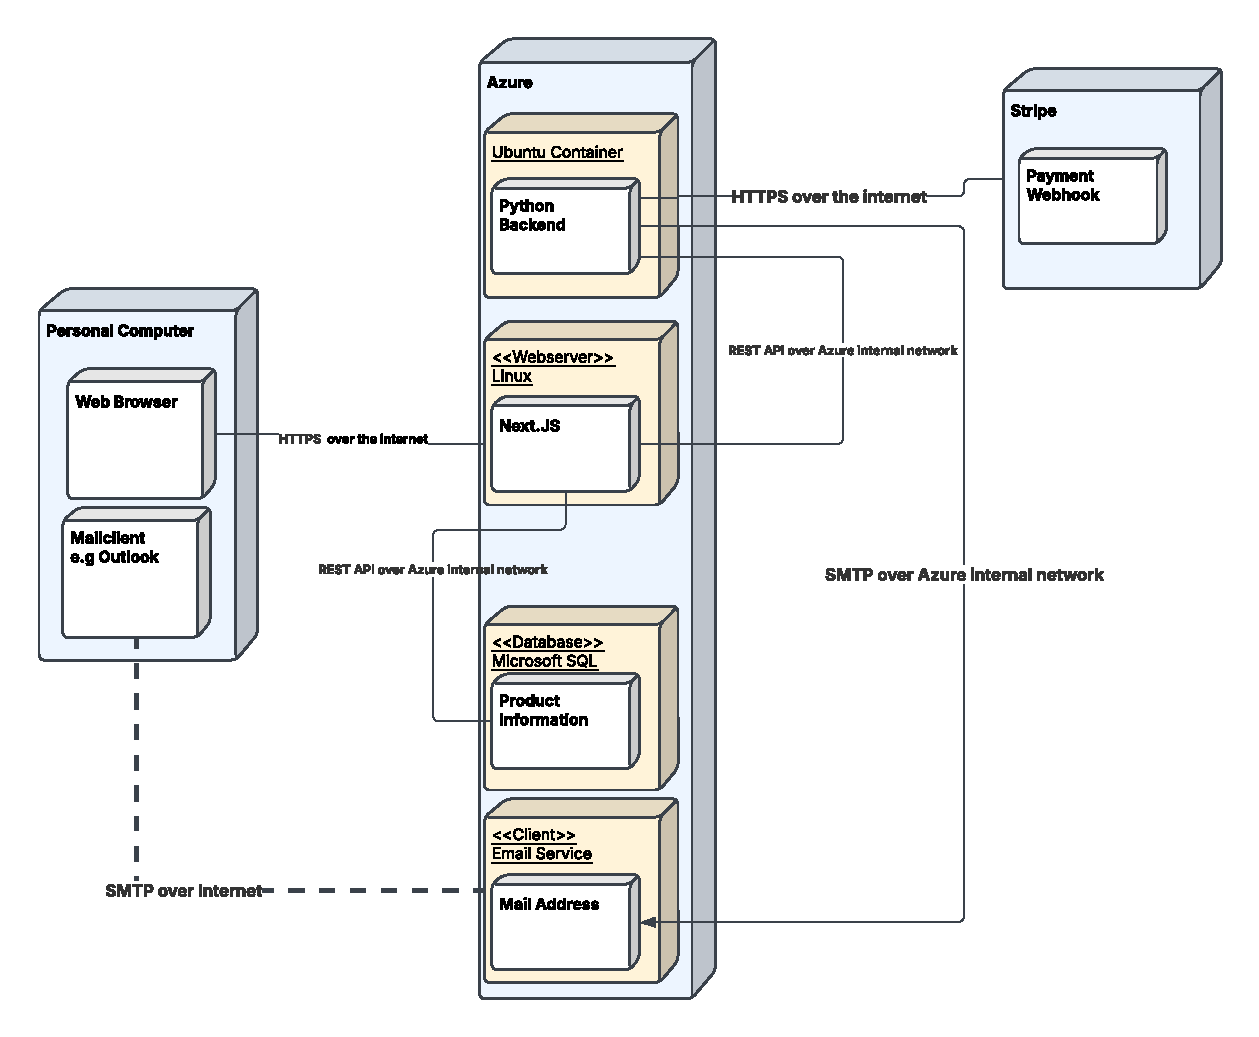
\includegraphics[width=0.8\textwidth]{images/webshop_deployment_diagram.pdf} 
  \caption{UML Deployment Diagram of the Webshop Technical Architecture}
  \label{fig:webshop-deployment}
\end{figure}

\begin{table}[h]
  \centering
  \resizebox{\textwidth}{!}{%
    \begin{tabular}{|l|l|l|}
      \hline
      Input/Output                          & Channel/Protocol               & Description (Optional)                   \\
      \hline
      Product requests, order details, payment info (Users → Webshop) & HTTPS over the Internet        & User interactions via web browser       \\
      Product listings, order confirmation (Webshop → Users) & HTTPS over the Internet        & Web app responses                        \\
      Product data, order storage requests (Webshop → Azure Database) & REST API over Azure internal network & Database queries and updates            \\
      Product info (Azure Database → Webshop) & REST API over Azure internal network & Data retrieval for product display      \\
      Payment info (Backend → Stripe)       & HTTPS over the Internet        & Payment processing requests             \\
      Payment webhook (Stripe → Backend)    & HTTPS over the Internet        & Payment status updates via webhook       \\
      Order details (Webshop → Azure Email Service) & SMTP over Azure internal network & Email notification setup                \\
      Email delivered to users (Azure Email Service → Users) & SMTP over Internet             & Email delivery to users                 \\
      \hline
    \end{tabular}
  }
  \caption{Mapping of Webshop Inputs/Outputs to Technical Channels}
  \label{tab:webshop-technical-mapping}
\end{table}
\newpage
\hypertarget{section-solution-strategy}{%
\section{Solution Strategy}\label{section-solution-strategy}}

\textbf{Contents}

A short summary and explanation of the fundamental decisions and
solution strategies, that shape system architecture. It includes

\begin{itemize}
\item
  technology decisions
\item
  decisions about the top-level decomposition of the system, e.g. usage
  of an architectural pattern or design pattern
\item
  decisions on how to achieve key quality goals
\item
  relevant organizational decisions, e.g. selecting a development
  process or delegating certain tasks to third parties.
\end{itemize}

\textbf{Motivation}

These decisions form the cornerstones for your architecture. They are
the foundation for many other detailed decisions or implementation
rules.

\textbf{Form}

Keep the explanations of such key decisions short.

Motivate what was decided and why it was decided that way, based upon
problem statement, quality goals and key constraints. Refer to details
in the following sections.

See \href{https://docs.arc42.org/section-4/}{Solution Strategy} in the
arc42 documentation.
\newpage
\hypertarget{section-building-block-view}{%
\section{5 Building Block View}\label{section-building-block-view}}

\textbf{Content}

This section shows the static decomposition of the system into building blocks (e.g. modules, components, subsystems, classes, interfaces, packages, libraries, frameworks, layers, partitions, tiers, functions, operations, \ldots) including their relationships and associations. It helps to maintain an overview of your source code by making its structure understandable through abstraction.

\subsection{Frontend}
\subsubsection{Component-Based Frontend Architecture}
The Vivendo webshop frontend follows a \textbf{component-based modular frontend design}. The different modules are interconnected to provide a seamless shopping experience. The primary technologies used include \textbf{Next.js, Tailwind CSS}, API integration and Context API for state management. This approach ensures:
\begin{itemize}
    \item Clear separation of concerns through distinct modules.
    \item Reusability of components across different sections.
    \item Better maintainability and scalability.
    \item Efficient state and API management.
\end{itemize}
The architectural overview is depicted in the figure below:

\begin{figure}[h]
    \centering
    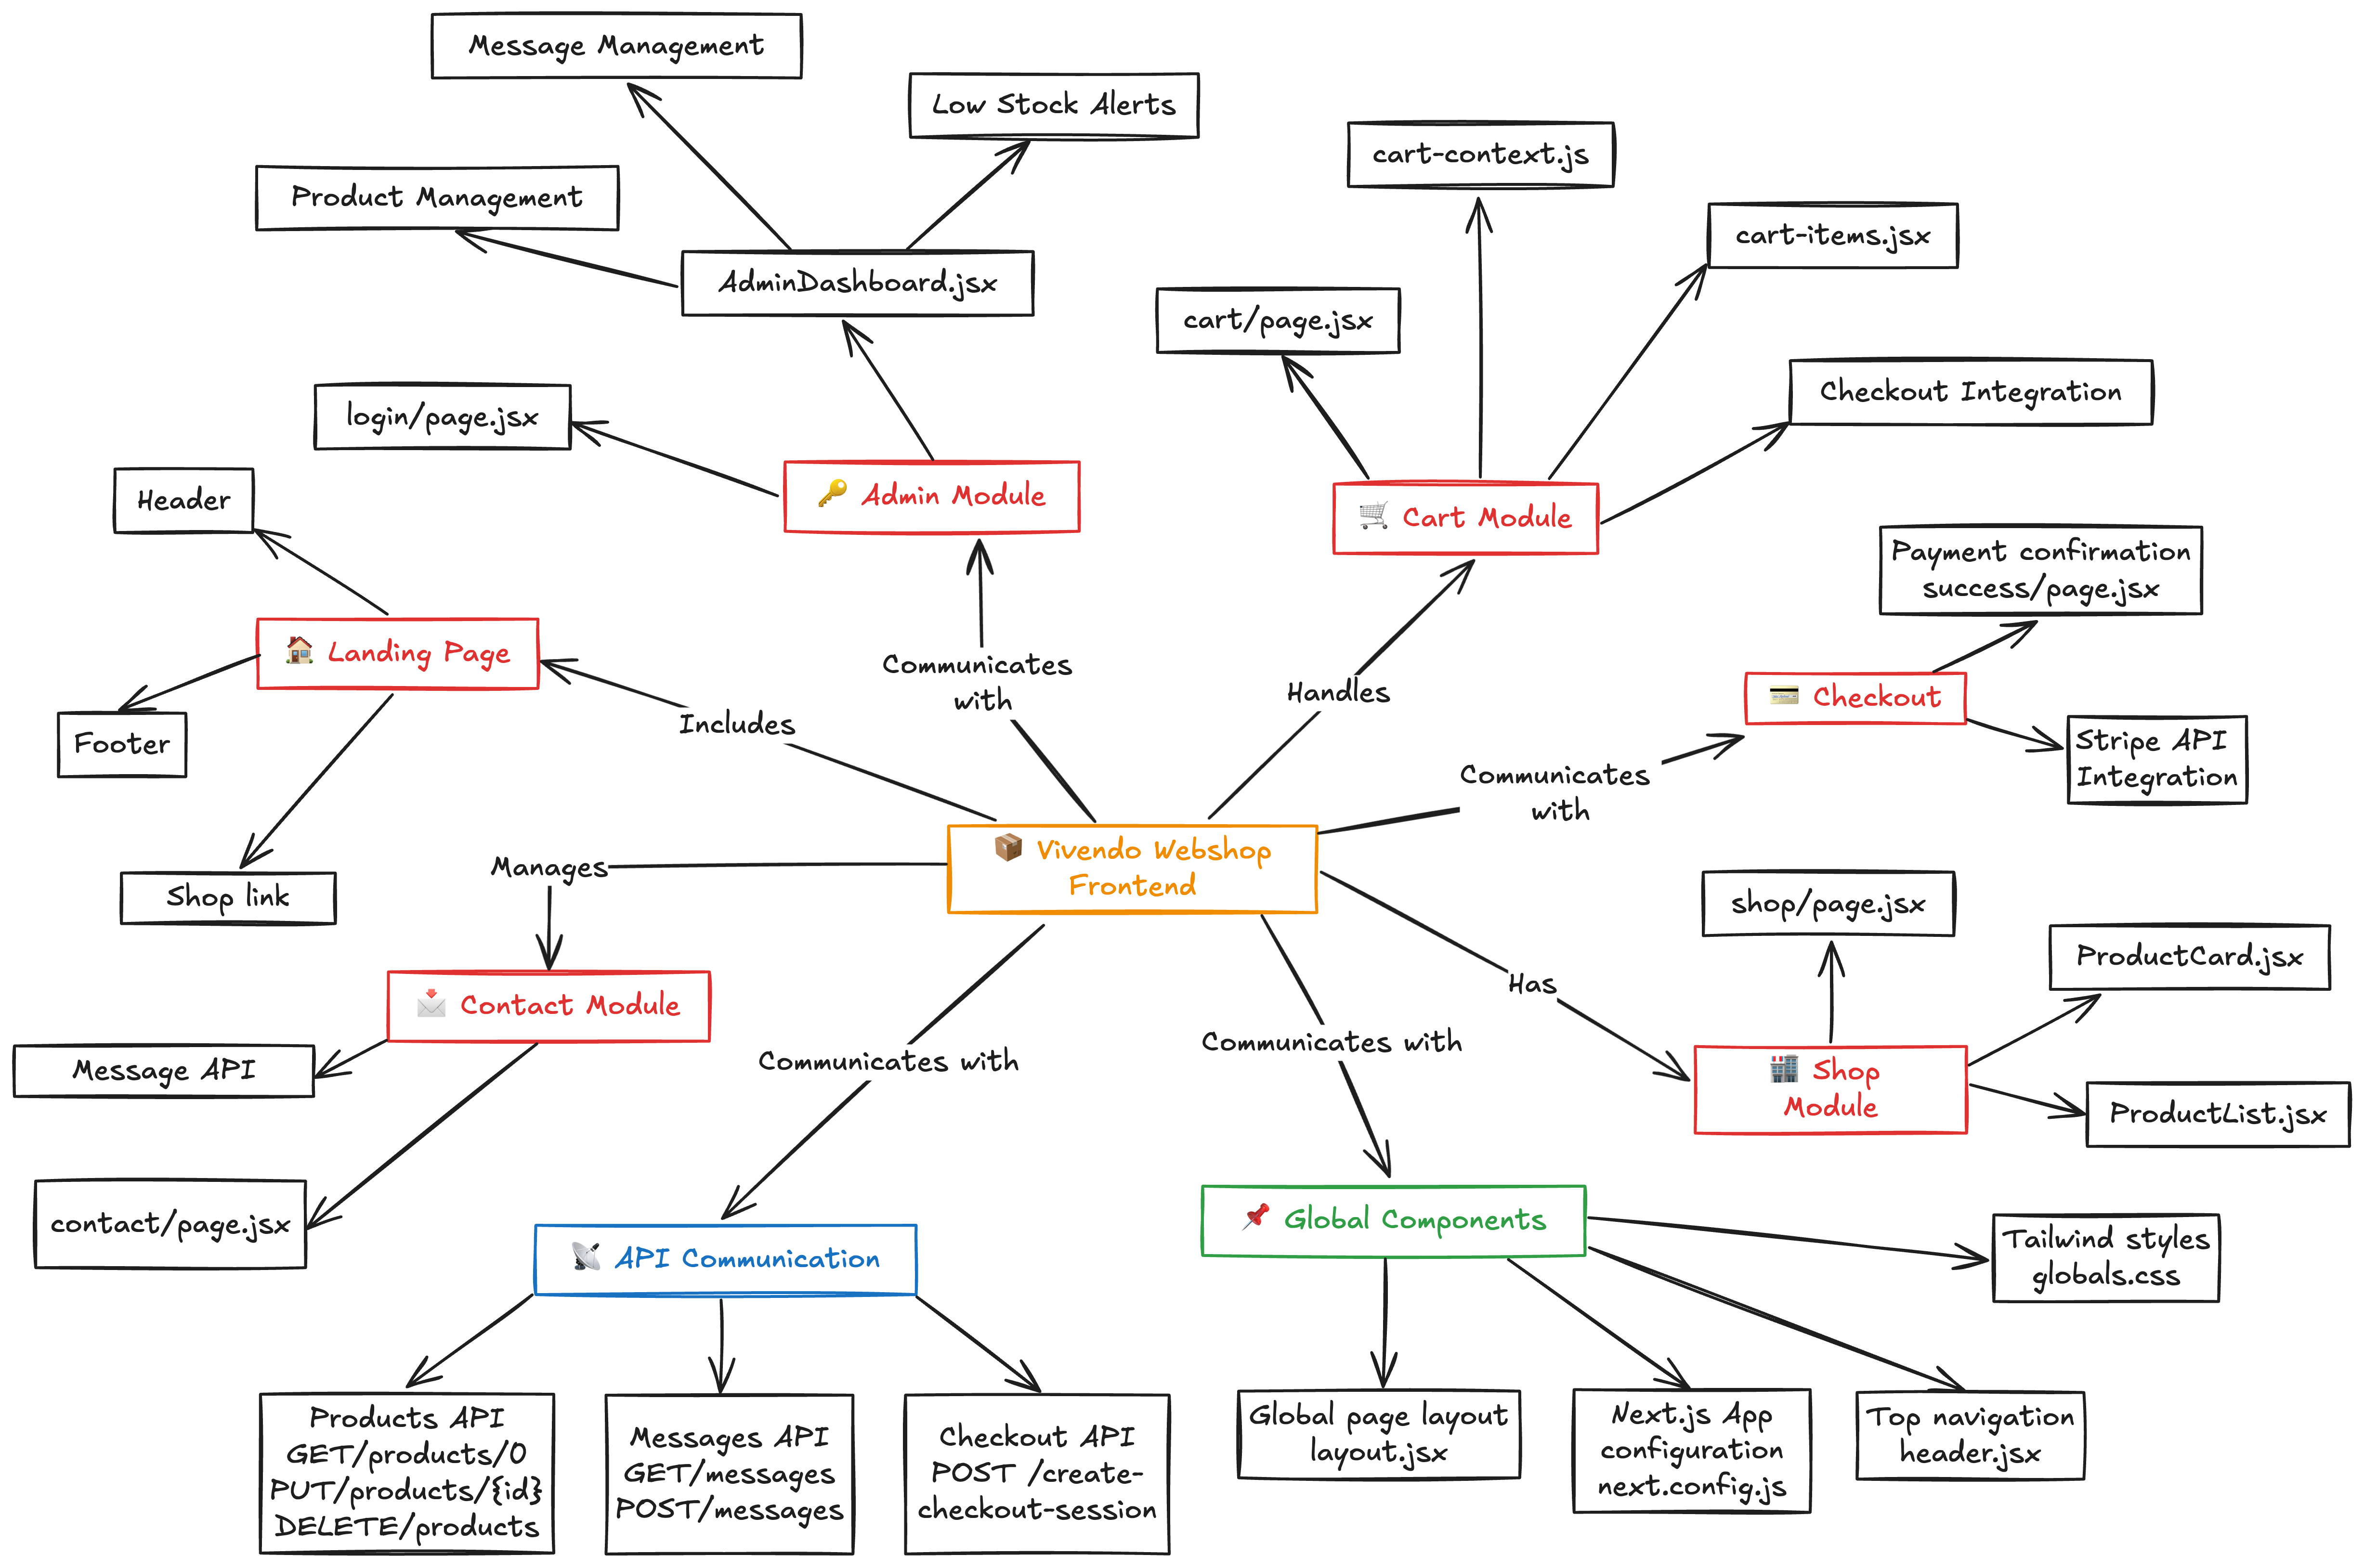
\includegraphics[width=\textwidth]{images/New_frontend_architecture.png}
    \caption{Component-Based Frontend Architecture}
    \label{fig:architecture}
\end{figure}

\subsubsection{Core Frontend Modules and Interactions}
The system consists of several modules:
\begin{itemize}
    \item \textbf{Landing Page Module}: Includes key UI components such as the header, footer and navigation links.
    \item \textbf{Admin Module}: Manages the admin dashboard, including product management, low stock alerts and message management. The admin module is responsible for managing products, messages, and stock alerts. It is connected to the \textbf{Admin Dashboard} component, which communicates with the API layer.
    \item \textbf{Cart Module}: Handles cart functionality, including cart context, cart items and checkout integration. The cart module manages cart-related functionalities and state using \texttt{cart-context.js}. It also connects with the checkout module to handle Stripe payments.
    \item \textbf{Shop Module}: Displays product listings and product cards with interactivity.
    \item \textbf{Checkout Module}: Integrates with Stripe API for handling payments and success confirmations.
    \item \textbf{Contact Module}: Manages user interactions via the contact page and handles message submissions. It connects with the API layer to store and retrieve messages.
    \item \textbf{API Communication Layer}: Manages requests to the backend services, including product APIs, messages API and checkout API. This layer serves as the middleware between the frontend and backend, making requests via REST APIs. It handles product data, message submissions, and checkout sessions.
    \item \textbf{Global Components}: Includes shared layout elements, styles and configurations.
\end{itemize}


%% ADD BACKEND BUILDING BLOCK VIEW PART / ARCHITECTURE HERE

\subsection{Backend}
\newpage
\hypertarget{section-runtime-view}{%
\section{Runtime View}\label{section-runtime-view}}

\textbf{Contents}

The runtime view describes concrete behavior and interactions of the
system's building blocks in form of scenarios from the following areas:

\begin{itemize}
\item
  important use cases or features: how do building blocks execute them?
\item
  interactions at critical external interfaces: how do building blocks
  cooperate with users and neighboring systems?
\item
  operation and administration: launch, start-up, stop
\item
  error and exception scenarios
\end{itemize}

Remark: The main criterion for the choice of possible scenarios
(sequences, workflows) is their \textbf{architectural relevance}. It is
\textbf{not} important to describe a large number of scenarios. You
should rather document a representative selection.

\textbf{Motivation}

You should understand how (instances of) building blocks of your system
perform their job and communicate at runtime. You will mainly capture
scenarios in your documentation to communicate your architecture to
stakeholders that are less willing or able to read and understand the
static models (building block view, deployment view).

\textbf{Form}

There are many notations for describing scenarios, e.g.

\begin{itemize}
\item
  numbered list of steps (in natural language)
\item
  activity diagrams or flow charts
\item
  sequence diagrams
\item
  BPMN or EPCs (event process chains)
\item
  state machines
\item
  \ldots{}
\end{itemize}

See \href{https://docs.arc42.org/section-6/}{Runtime View} in the arc42
documentation.

\hypertarget{__runtime_scenario_1}{%
\subsection{\textless Runtime Scenario
1\textgreater{}}\label{__runtime_scenario_1}}

\begin{itemize}
\item
  \emph{\textless insert runtime diagram or textual description of the
  scenario\textgreater{}}
\item
  \emph{\textless insert description of the notable aspects of the
  interactions between the building block instances depicted in this
  diagram.\textgreater{}}
\end{itemize}

\hypertarget{__runtime_scenario_2}{%
\subsection{\textless Runtime Scenario
2\textgreater{}}\label{__runtime_scenario_2}}

\hypertarget{_}{%
\subsection{\ldots{}}\label{_}}

\hypertarget{__runtime_scenario_n}{%
\subsection{\textless Runtime Scenario
n\textgreater{}}\label{__runtime_scenario_n}}
\newpage
\hypertarget{section-deployment-view}{%
\section{Deployment View}\label{section-deployment-view}}

\hypertarget{_infrastructure_level_1}{%
\subsection{Microsoft Azure Deployment}\label{_infrastructure_level_1}}

\begin{figure}[h]
  \centering
  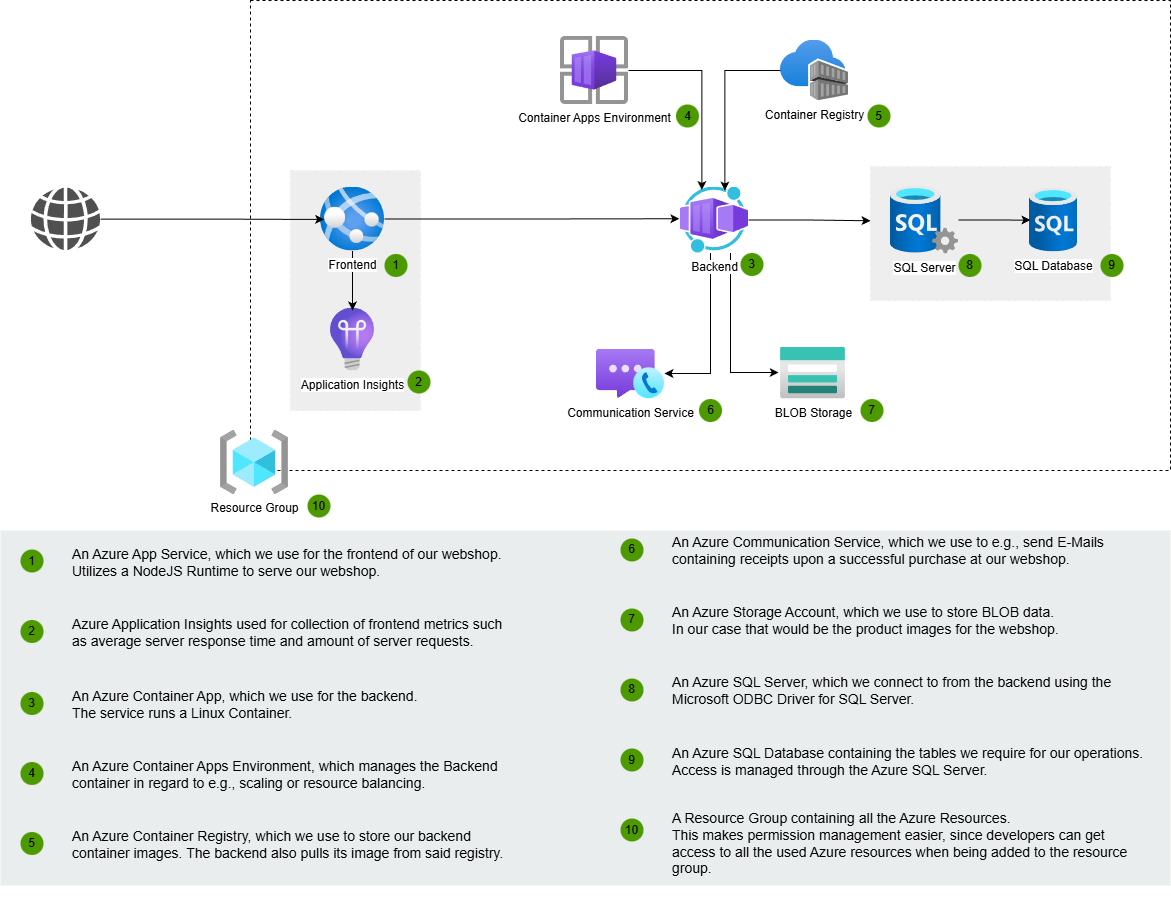
\includegraphics[width=\textwidth]{images/azure_deployment_view.png}
  \caption{Azure Infrastructure Diagram}
\end{figure}

\subsubsection{Motivation}
Instead of hosting the application locally on-premise, we instead opted for hosting it on the cloud.
This has multiple advantages such as not having to manage our own hardware as well as allowing more efficient resource utilization
by using a pay-as-you-go method of billing, rather than investing into our own hardware outright.

We chose to go forward with Microsoft Azure as our Cloud Service Provider, because they offer advanced features,
which we can make good use of, 
being reliable and easy to deploy with.

Now follow rationales for select services, where multiple Azure offerings could have been considered instead.

\begin{longtable}[]{@{}
  >{\raggedright\arraybackslash}p{(\columnwidth - 2\tabcolsep) * \real{0.3333}}
  >{\raggedright\arraybackslash}p{(\columnwidth - 2\tabcolsep) * \real{0.6667}}@{}}
\toprule
\begin{minipage}[b]{\linewidth}\raggedright
\textbf{Component}
\end{minipage} & \begin{minipage}[b]{\linewidth}\raggedright
\textbf{Rationale}
\end{minipage} \\
\midrule
\endhead
Frontend &
The frontend is served using NodeJS, therefore we deployed it using an Azure App Service,
since that is the most convenient way of deploying NodeJS applications on Azure. 
\\ \hline
Backend &
The python backend was designed as a Docker container in order to have e.g., rather simple horizontal scaling.
Therefore, it is suitable to use an Azure Container App to deploy the container into the cloud.
\\ \hline
Database &
As our database, we are utilizing the SaaS offering of Azure SQL Database, since it is generally more reliable
and more comfortable to work with, compared to hosting your own database with a PaaS offering.
Furthermore, we have personal preference toward managing relational databases, rather than non-relational databases.
Otherwise, we could have opted for non-relational database SaaS offering such as Azure Cosmos DB.
\\
\bottomrule
\end{longtable}

\subsubsection{Quality and/or Performance Features}
\begin{longtable}[]{@{}
  >{\raggedright\arraybackslash}p{(\columnwidth - 2\tabcolsep) * \real{0.3333}}
  >{\raggedright\arraybackslash}p{(\columnwidth - 2\tabcolsep) * \real{0.6667}}@{}}
\toprule
\begin{minipage}[b]{\linewidth}\raggedright
\textbf{Component}
\end{minipage} & \begin{minipage}[b]{\linewidth}\raggedright
\textbf{Quality and/or Performance Feature(s)}
\end{minipage} \\
\midrule
\endhead
Frontend &
The Azure App Service features 99.95\% guaranteed uptime as per the service-level agreement (SLA),
which is crucial for fulfilling our requirement of having high availability. 
\\ \hline
Backend &
The Azure Container App features the ability of creating replicas, allowing for horizontal scaling,
which can even be scaled automatically based on e.g., amount of concurrent incoming requests or CPU usage,
allowing for greater performance.
\\ \hline
Database &
The Azure SQL Database SaaS offering provides 99.99\% availability as per the service-level agreement.
This option allows for seamless upgrades to more premium service tiers, 
allowing for even availability guarantees exceeding 99.99\%.
Furthermore, more premium service tiers allow for using features, such as geo-redundant backup storage,
which replicates additional backups to a physical location hundreds of miles away from the primary region,
making it even more unlikely to lose significant amounts of data, even in catastrophic cases.
\\ \hline
BLOB Storage &
With Azure Storage Accounts, which we use for the blob storage, we have a 99.9\% availability as per the service-level agreement.
More premium options allow for going as high as 99.99\% availability.
\\ \hline
Azure Communication Services &
Azure Communication Services have an availability of 99.9\% guaranteed availability as per the service-level agreement,
making it so that our mailing service is highly available.
\\
\bottomrule
\end{longtable}

\subsubsection{Mapping}
Now follows a mapping of components in the building block view to components in the deployment view:

\subsubsection{Quality and/or Performance Features}
\begin{longtable}[]{@{}
  >{\raggedright\arraybackslash}p{(\columnwidth - 2\tabcolsep) * \real{0.3333}}
  >{\raggedright\arraybackslash}p{(\columnwidth - 2\tabcolsep) * \real{0.6667}}@{}}
\toprule
\begin{minipage}[b]{\linewidth}\raggedright
\textbf{Component in Building Block View}
\end{minipage} & \begin{minipage}[b]{\linewidth}\raggedright
\textbf{Component in Deployment View}
\end{minipage} \\
\midrule
\endhead
Frontend & 
\begin{itemize}
  \item App Service
  \item Application Insights
\end{itemize} \\ \hline
Backend & 
\begin{itemize}
  \item Container App
  \item Container Apps Environment
  \item Container Registry
\end{itemize} \\ \hline
E-Mail Service &
\begin{itemize}
  \item Communication Service
\end{itemize} \\ \hline
Database &
\begin{itemize}
  \item SQL Server
  \item SQL Database
\end{itemize} \\ \hline
\bottomrule
Image Storage &
\begin{itemize}
  \item Storage Account
\end{itemize} \\
\bottomrule
\end{longtable}\newpage
\hypertarget{section-concepts}{%
\section{8 Crosscutting Concepts and Architectural Decisions}\label{section-concepts}}

\textbf{Content}

This section describes overall, principal regulations and solution ideas that are relevant in multiple parts (= crosscutting) of our system and its architecture. Such concepts and decisions are often related to multiple building blocks and can include many different topics, such as

\begin{itemize}
\item
  models, especially domain models
\item
  architecture or design patterns
\item
  rules for using specific technology
\item
  principal, often technical decisions of an overarching nature
\item
  implementation rules
\end{itemize}

\subsection{Domain Model \& Data Structures}
The Vivendo Webshop frontend relies on several key data models that keep information consistent across different parts of the application:

\begin{itemize}
  \item \textbf{Product Model}: This structure includes fields such as the product ID, name, description, price, and stock level. Any part of the webshop that displays or updates product information---including the Shop Module and the Admin Dashboard---uses this same model.
  
  \item \textbf{Cart Item Model}: This extends the Product Model by incorporating cart-related details, such as quantity or item-level notes. The Cart Context employs this structure to ensure that updates to product attributes, like pricing or availability, remain in sync with a user's cart.
  
  \item \textbf{Message Model}: This standardized format describes user inquiries with fields such as subject, sender information, and message text. Both the Contact Module and the Admin Dashboard interact with this single model to create, display, and manage messages consistently.
\end{itemize}

We maintain these data models as shared sources of truth (SSOT). Splitting them into different product models for the shop and the admin area would risk creating mismatches if one model would be updated without the other. It would also complicate maintenance, since any field changes would need to be replicated in multiple places. By using these core structures throughout the system, we reduce the likelihood of data inconsistencies and simplify ongoing feature development.

\subsection{UI \& UX Conventions}
All pages in the Vivendo Webshop share a unified layout and design language. A global layout component (\texttt{layout.jsx}) includes site-wide elements such as the header, footer and navigation links. This approach guarantees that the user experience remains consistent across all modules. Tailwind CSS is used to provide a utility-first styling approach so that developers can quickly apply spacing, color, and typography classes to maintain uniform visuals. 

We selected Tailwind because of its flexibility and the minimal overhead it adds, Although other frameworks like Bootstrap might provide predefined components, those often require extensive overrides to achieve a specific kind of identity. 

\subsection{Routing \& Folder Structure (Next.js)}
Our Next.js setup uses file-based routing to map files within the \texttt{pages/} directory to distinct routes. This arrangement makes the URL structure predictable for both developers and users. Public pages - including the shop, cart, and contact form - reside under straightforward displayed paths, while administrative features such as login or the Admin Dashboard are kept separate to detach sensitive functionality.

We chose Next.js because it offers server-side rendering and built-in image optimization. These features are valuable for an online shop (e.g. Vivendo) where both SEO and performance are important. Besides alternative solutions, Next.js fits best with the platform's requirement for dynamic content, simple configuration and a strong user experience across devices.

\subsection{Shared State Management}
React Context API is used to share and manage global data. For example, the Cart Context holds a user’s cart items and provides methods to add, remove, or update them. By centralizing cart logic, all components in the webshop - from product pages to checkout flows - operate on the same state and can render consistent information. 

\subsection{Security \& Authentication}
The webshop uses an authentication-based route for the dashboard including all administrative features. This ensures that unauthorized individuals cannot edit products or read messages. The current approach checks whether the username and password match the required values and if valid, stores them in a local storage to simulate a logged-in state. This design is sufficient for a simple prototype but would need to be replaced with a more secure solution in a production environment.

For payment processing the system depends on Stripe to handle sensitive credit card data. This reliance on a secure external provider reduces compliance overhead for our team and limits the exposure of critical payment details in our infrastructure. We selected Stripe based on its popularity, strong security posture and clear documentation for the integration with Next.js. 

\subsection{Error Handling \& Logging}
React error boundaries catch unexpected exceptions in key components, preventing the entire application from failing if one feature encounters a problem. 

\subsection{Consolidated Architectural Decisions}
\begin{itemize}
  \item \textbf{Next.js} is our framework for delivering server-rendered pages and handling routing automatically.
  \item \textbf{Stripe} is used for payment processing, removing the need to manage credit card data in our own systems.
  \item \textbf{React Context} manages global state, such as the shopping cart, in order to reduce boilerplate and maintain clarity.
  \item \textbf{Single Source of Truth} for data models avoids the duplication of field definitions across modules.
\end{itemize}

These decisions ensure that the our frontend remains flexible and performant through maintaining an architecture that is adaptable as the platform evolves.\newpage
\hypertarget{section-quality-scenarios}{%
\section{9 Quality Requirements}\label{section-quality-scenarios}}

\textbf{Contents}

This section details the quality requirements for the Webshop system, focusing on performance, security, usability, maintainability, and reliability. It includes a quality tree to prioritize these attributes and quality scenarios to make them concrete and measurable, covering both critical goals (e.g., security) and lower-priority ones (e.g., reliability).

\textbf{Motivation}

Quality requirements are essential for the Webshop to meet user expectations, ensure reliable operation, and support future growth. They guide architectural decisions about cloud infrastructure, payment integration, and user interface design, ensuring the system is secure, performant, and user-friendly for users.

\hypertarget{_quality_tree}{%
\subsection{Quality Tree}\label{_quality_tree}}

\textbf{Contents}
The quality tree organizes the Webshop’s quality attributes, starting with ‘Quality’ as the root and branching into categories like Performance, Security, Usability, Maintainability, and Reliability, with sub-attributes and priorities linked to quality scenarios. It reflects both normal operating conditions and peak demand scenarios to ensure comprehensive coverage.

\textbf{Motivation}
The quality tree provides a structured overview and prioritization of the Webshop’s quality requirements, helping Developers focus on critical aspects like security and performance while addressing secondary goals like usability and system reliability. It enables architects to evaluate and design the system effectively, linking to detailed scenarios for validation.

\textbf{Form}
The quality tree is presented as a hierarchical diagram, with ‘Quality’ at the top-left, branching horizontally into categories and sub-attributes, each with priorities (High, Medium, Low) and references to corresponding quality scenarios in the Quality Scenarios section.

\begin{figure}[h]
  \centering
  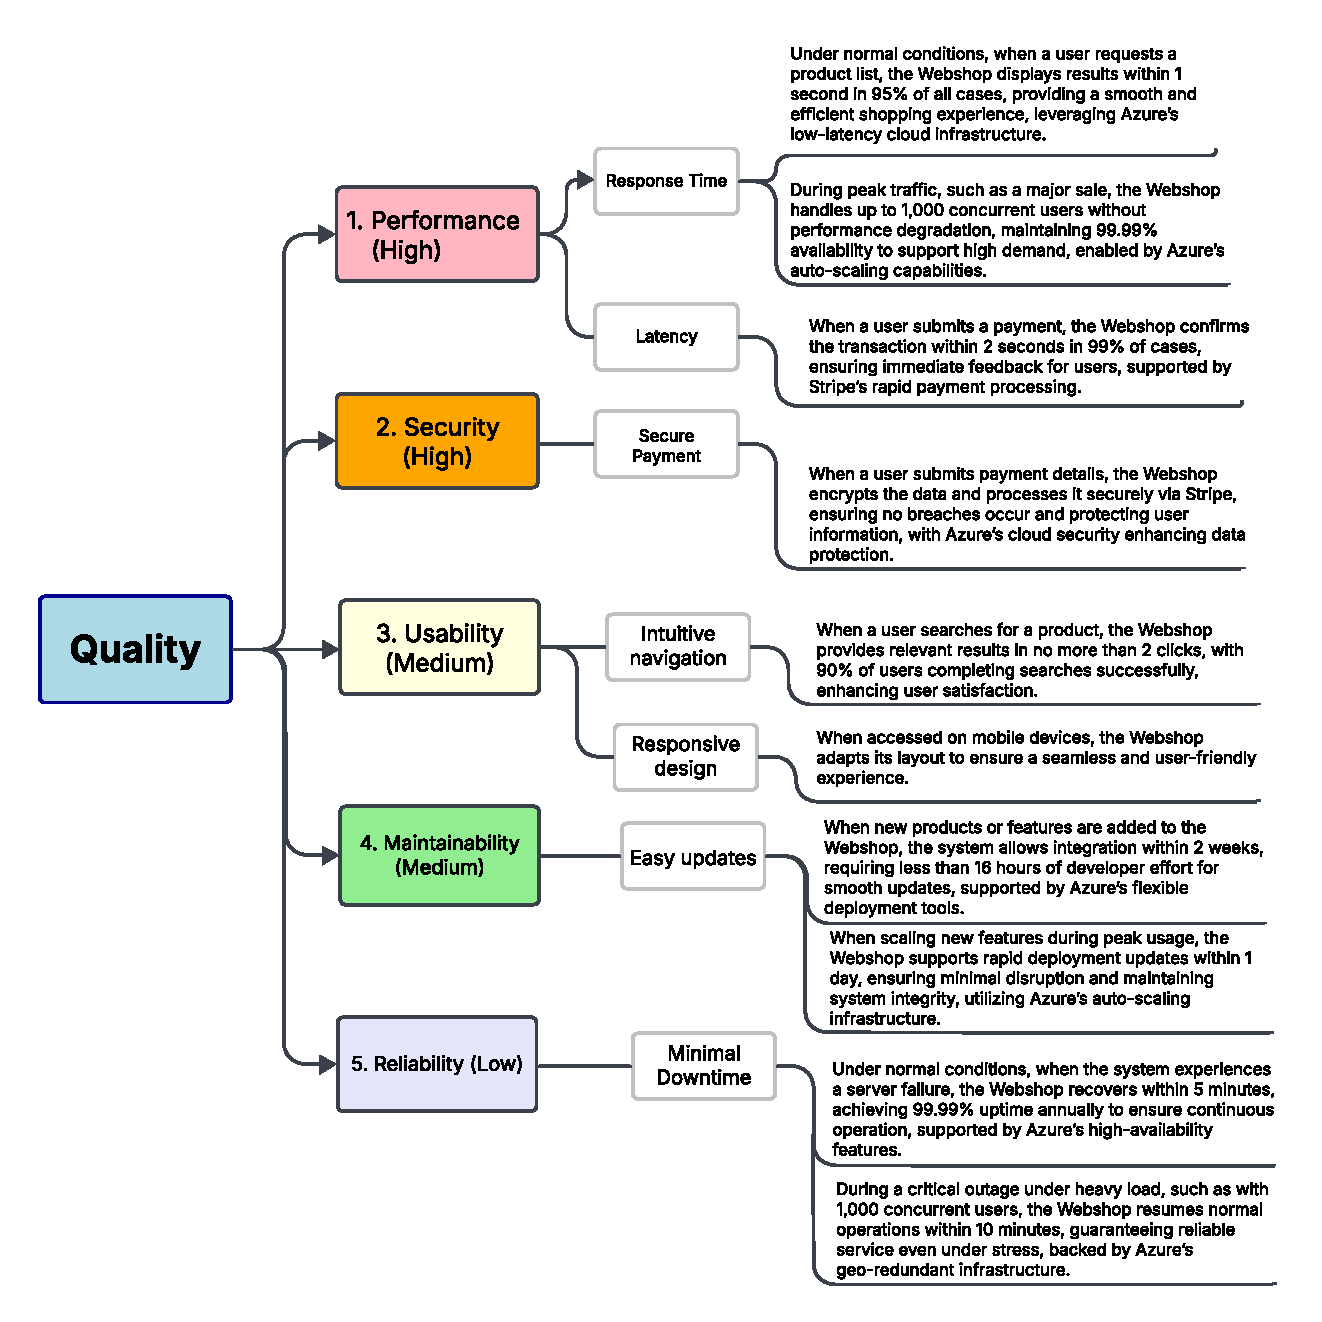
\includegraphics[width=0.9\textwidth]{images/quality-tree.pdf}
  \caption{Quality Tree for the Webshop System}
  \label{fig:webshop-quality-tree}
\end{figure}

\hypertarget{_quality_scenarios}{%
\subsection{Quality Scenarios}\label{_quality_scenarios}}

\textbf{Contents}

This subsection provides concrete quality scenarios for the Webshop, detailing runtime responses to stimuli (usage scenarios) and system modifications (change scenarios), with measures and priorities linked to the quality tree. It includes scenarios for both normal conditions and peak demand to ensure robust system performance.

\textbf{Motivation}

Quality scenarios make the Webshop’s quality requirements tangible, allowing architects to design and test for performance, security, usability, and reliability. They ensure the system meets user expectations, supports cloud-based operations and payment integration, and can be evaluated for trade-offs, providing clarity for Developers in development and evaluation.

\textbf{Form}

Quality scenarios are presented in a tabular format, with columns for scenario type, stimulus, response, measure, and priority, corresponding to leaves in the quality tree.

\begin{table}[h]
  \centering
  \renewcommand{\arraystretch}{1.2} 
  \setlength{\tabcolsep}{4pt} 
  \resizebox{\textwidth}{!}{ 
      \begin{tabular}{|p{3cm}|p{3cm}|p{4cm}|p{3cm}|c|}
          \hline
          \textbf{Scenario Type} & \textbf{Stimulus} & \textbf{Response} & \textbf{Measure} & \textbf{Priority} \\
          \hline
          Usage (Performance)  & User requests a product list & System displays products within 1 second & 95\% of requests complete in <1 second & High \\
          \hline
          Change (Performance)  & Traffic spikes during a sale & System handles 1,000 concurrent users & 99\% availability during peak load & High \\
          \hline
          Usage (Performance)  & User submits payment & System confirms transaction within 2 seconds & 99\% of transactions complete in <2 seconds & High \\
          \hline
          Usage (Security)  & User submits payment details & System encrypts data and processes via Stripe & Data encrypted with TLS 1.2, no breaches & High \\
          \hline
          Usage (Usability)  & User searches for a product & System shows relevant results in 2 clicks & 90\% of users complete searches successfully & Medium \\
          \hline
          Usage (Usability)  & User accesses Webshop on mobile & System adapts layout for mobile devices & 95\% of mobile users report satisfaction & Medium \\
          \hline
          Change (Maintainability)  & New products or features are added & System integrates within 2 weeks & Integration completed with <16 hours effort & Medium \\
          \hline
          Change (Maintainability)  & Scaling new features during peak usage & System integrates updates within 1 day & Integration completed with <24 hours effort & Medium \\
          \hline
          Usage (Reliability)  & System experiences server failure & System recovers within 5 minutes & 99.9\% uptime annually & Low \\
          \hline
          Usage (Reliability)  & System outage under heavy load & System resumes normal operations within 10 minutes & 99.9\% uptime during peak load & Low \\
          \hline
      \end{tabular}
  }
  \caption{Quality Scenarios for the Webshop System}
  \label{tab:webshop-quality-scenarios}
\end{table}


\end{document}\newpage
\hypertarget{section-technical-risks}{%
\section{Risks and Technical Debts}\label{section-technical-risks}}

\textbf{Contents}

A list of identified technical risks or technical debts, ordered by
priority

\textbf{Motivation}

``Risk management is project management for grown-ups'' (Tim Lister,
Atlantic Systems Guild.)

This should be your motto for systematic detection and evaluation of
risks and technical debts in the architecture, which will be needed by
management stakeholders (e.g. project managers, product owners) as part
of the overall risk analysis and measurement planning.

\textbf{Form}

List of risks and/or technical debts, probably including suggested
measures to minimize, mitigate or avoid risks or reduce technical debts.

See \href{https://docs.arc42.org/section-11/}{Risks and Technical Debt}
in the arc42 documentation.
\newpage
\hypertarget{section-glossary}{%
\section{Glossary}\label{section-glossary}}

\textbf{Contents}

The most important domain and technical terms that your stakeholders use
when discussing the system.

You can also see the glossary as source for translations if you work in
multi-language teams.

\textbf{Motivation}

You should clearly define your terms, so that all stakeholders

\begin{itemize}
\item
  have an identical understanding of these terms
\item
  do not use synonyms and homonyms
\end{itemize}

A table with columns \textless Term\textgreater{} and
\textless Definition\textgreater.

Potentially more columns in case you need translations.

See \href{https://docs.arc42.org/section-12/}{Glossary} in the arc42
documentation.

\begin{longtable}[]{@{}
  >{\raggedright\arraybackslash}p{(\columnwidth - 2\tabcolsep) * \real{0.3333}}
  >{\raggedright\arraybackslash}p{(\columnwidth - 2\tabcolsep) * \real{0.6667}}@{}}
\toprule
\begin{minipage}[b]{\linewidth}\raggedright
Term
\end{minipage} & \begin{minipage}[b]{\linewidth}\raggedright
Definition
\end{minipage} \\
\midrule
\endhead
\emph{Cloud Service Provider (CSP)} &
\emph{A Cloud Service Provider (CSP) is a third-party company, 
which offers (paid) services in regard to cloud capabilities, be it compute, storage, management, and/or analytics. 
In our case, we are solely referring to public Cloud Service Providers, which provide these services to the public,
opposed to offering services exclusive to one or multiple companies.} \\ \hline
\emph{Microsoft Azure ("Azure")} &
\emph{Microsoft Azure is a public cloud service provider belonging to Microsoft.} \\ \hline
\emph{Service-Level Agreement (SLA)} &
\emph{Service-level agreements are made between a (cloud) service provider and a customer. 
For our purposes, the main point of interest, is availability, where the (cloud) service provider
guarantees a certain availability for a given service, 
allowing us to fulfill our own availability requirements when relying on said service.} \\ \hline
\emph{Horizontal Scaling} &
\emph{Horizontal Scaling refers to improving performance by spinning up multiple instances,
so that requests can be distributed among them, allowing for greater parallel processing, 
rather than just increasing hardware performance directly (Vertical Scaling).} \\ \hline
\emph{Replica} &
\emph{A replica in our case refers to additional copies of either Docker containers or database copies.
The purpose is to provide increased performance (horizontal scaling), such as having multiple read-only replicas of a database, 
allowing for higher throughput of read operations, 
especially if additional replicas are spread geographically to decrease latency.
Replicas also increases availability, especially if they are spread geographically, 
making it so that an instance of a service is running even if there were to be a data center failure at N-1 locations.} \\
\bottomrule
\end{longtable}
\newpage
\hypertarget{section-information-about-work}{%
\section{12 Information about Work}\label{section-information-about-work}}

\subsection{Distribution of Report Work}
\begin{longtable}[]{@{}
    >{\raggedright\arraybackslash}p{(\columnwidth - 2\tabcolsep) * \real{0.3333}}
    >{\raggedright\arraybackslash}p{(\columnwidth - 2\tabcolsep) * \real{0.6667}}@{}}
\toprule
\begin{minipage}[b]{\linewidth}\raggedright
\textbf{Member}
\end{minipage} & \begin{minipage}[b]{\linewidth}\raggedright
\textbf{Sections}
\end{minipage} \\
\midrule
\endhead
Vinay Duhan &
\begin{itemize}
    \item 1- Introduction and Goals
    \item 2- Constraints
\end{itemize} \\ \hline
Jatender Singh Jossan &
\begin{itemize}
    \item 4- Solution Strategy
    \item 5- Building Block View (Frontend, Backend side)
    \item 8- Crosscutting Concepts
\end{itemize} \\ \hline
Dennis Mark &
\begin{itemize}
    \item 4- Solution Strategy
    \item 5- Building Block View (Frontend side)
    \item 8- Crosscutting Concepts
\end{itemize} \\ \hline
Dominique Conceicao Rosario &
\begin{itemize}
    \item 3- Context and Scope
    \item 5- Building Block View (Backend side)
    \item 10- Quality Requirements
    \item 11- Risks and Technical Debt
\end{itemize} \\ \hline
Edward Späth &
\begin{itemize}
    \item 5- Building Block View (Backend and Database)
    \item 6- Runtime View
    \item 7- Deployment View
\end{itemize} \\
\bottomrule
\end{longtable}

\subsection{Repository}
The public GitHub Repository is online and can be reached at 
\url{https://github.com/EdwardSpaeth/Cloud-Project-Group-11}.
The GitHub usernames can be mapped to each project member in the following way:

\begin{longtable}[]{@{}
    >{\raggedright\arraybackslash}p{(\columnwidth - 2\tabcolsep) * \real{0.3333}}
    >{\raggedright\arraybackslash}p{(\columnwidth - 2\tabcolsep) * \real{0.6667}}@{}}
\toprule
\begin{minipage}[b]{\linewidth}\raggedright
\textbf{Member}
\end{minipage} & \begin{minipage}[b]{\linewidth}\raggedright
\textbf{GitHub Username}
\end{minipage} \\
\midrule
\endhead
Vinay Duhan & duhanvinay \\ \hline
Jatender Singh Jossan & jatenderjossan \\ \hline
Dennis Mark & solipskierr \\ \hline
Dominique Conceicao Rosario & DomiRosario \\ \hline
Edward Späth & EdwardSpaeth \\
\bottomrule
\end{longtable}


\end{document}
